\documentclass{article}\usepackage[]{graphicx}\usepackage[]{xcolor}
% maxwidth is the original width if it is less than linewidth
% otherwise use linewidth (to make sure the graphics do not exceed the margin)
\makeatletter
\def\maxwidth{ %
  \ifdim\Gin@nat@width>\linewidth
    \linewidth
  \else
    \Gin@nat@width
  \fi
}
\makeatother

\definecolor{fgcolor}{rgb}{0.345, 0.345, 0.345}
\newcommand{\hlnum}[1]{\textcolor[rgb]{0.686,0.059,0.569}{#1}}%
\newcommand{\hlsng}[1]{\textcolor[rgb]{0.192,0.494,0.8}{#1}}%
\newcommand{\hlcom}[1]{\textcolor[rgb]{0.678,0.584,0.686}{\textit{#1}}}%
\newcommand{\hlopt}[1]{\textcolor[rgb]{0,0,0}{#1}}%
\newcommand{\hldef}[1]{\textcolor[rgb]{0.345,0.345,0.345}{#1}}%
\newcommand{\hlkwa}[1]{\textcolor[rgb]{0.161,0.373,0.58}{\textbf{#1}}}%
\newcommand{\hlkwb}[1]{\textcolor[rgb]{0.69,0.353,0.396}{#1}}%
\newcommand{\hlkwc}[1]{\textcolor[rgb]{0.333,0.667,0.333}{#1}}%
\newcommand{\hlkwd}[1]{\textcolor[rgb]{0.737,0.353,0.396}{\textbf{#1}}}%
\let\hlipl\hlkwb

\usepackage{framed}
\makeatletter
\newenvironment{kframe}{%
 \def\at@end@of@kframe{}%
 \ifinner\ifhmode%
  \def\at@end@of@kframe{\end{minipage}}%
  \begin{minipage}{\columnwidth}%
 \fi\fi%
 \def\FrameCommand##1{\hskip\@totalleftmargin \hskip-\fboxsep
 \colorbox{shadecolor}{##1}\hskip-\fboxsep
     % There is no \\@totalrightmargin, so:
     \hskip-\linewidth \hskip-\@totalleftmargin \hskip\columnwidth}%
 \MakeFramed {\advance\hsize-\width
   \@totalleftmargin\z@ \linewidth\hsize
   \@setminipage}}%
 {\par\unskip\endMakeFramed%
 \at@end@of@kframe}
\makeatother

\definecolor{shadecolor}{rgb}{.97, .97, .97}
\definecolor{messagecolor}{rgb}{0, 0, 0}
\definecolor{warningcolor}{rgb}{1, 0, 1}
\definecolor{errorcolor}{rgb}{1, 0, 0}
\newenvironment{knitrout}{}{} % an empty environment to be redefined in TeX

\usepackage{alltt}
\usepackage{amsmath} %This allows me to use the align functionality.
                     %If you find yourself trying to replicate
                     %something you found online, ensure you're
                     %loading the necessary packages!
\usepackage{amsfonts}%Math font
\usepackage{graphicx}%For including graphics
\usepackage{hyperref}%For Hyperlinks
\usepackage[shortlabels]{enumitem}% For enumerated lists with labels specified, % We had to run tlmgr_install("enumitem") in R
\hypersetup{colorlinks = true,citecolor=black} %set citations to have black (not green) color
\usepackage{natbib}        %For the bibliography
\setlength{\bibsep}{0pt plus 0.3ex}
\bibliographystyle{apalike}%For the bibliography
\usepackage[margin=0.50in]{geometry}
\usepackage{float}
\usepackage{multicol}

%fix for figures
\usepackage{caption}
\newenvironment{Figure}
  {\par\medskip\noindent\minipage{\linewidth}}
  {\endminipage\par\medskip}
\IfFileExists{upquote.sty}{\usepackage{upquote}}{}
\begin{document}

\vspace{-1in}
\title{Lab 10 -- MATH 240 -- Computational Statistics}

\author{
  Anya Suko\\
}

\date{April 10, 2024}

\maketitle

\begin{multicols}{2}
%\raggedcolumns % If your spacing gets messed up try uncommenting 
                % this line

\section{Introduction}
In this lab, we examine Gallup's study on polling. The study explains that a poll of 1,000 people can have a margin of error of 4 percent, while a poll of 2,000 people can reduce that margin to 2. Our objective in this lab is to run simulations to better understand how sample size impacts the margin of error and compare our results to Gallup's findings. We also look at re sampling and other methods to see how different factors, like sample size and population proportion, influence the margin of error, helping us understand how Gallup improves its polling accuracy. 

\section{Basic Simulation}
First, we conducted a basic simulation of 10,000 polls using a sample size of 1,004. For the population, we assume 0.39 is the proportion of satisfied respondents.We use a binomial distribution to model the responses.

\begin{Figure}
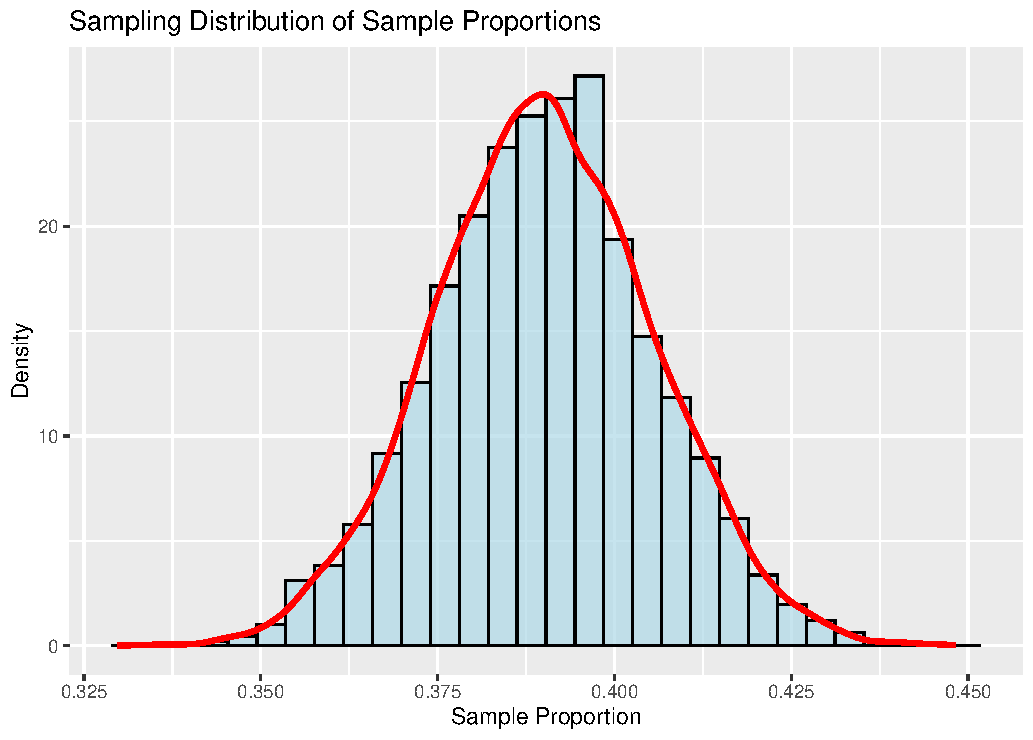
\includegraphics[width=\linewidth]{plot 1.pdf}
\captionof{figure}{Basic Simulation with size 1,004 }
\end{Figure}

The distribution is bell shaped and symmetric. The middle 95 percent of the data ranges from approximately [0.3613, 0.4181], which has a margin of error of 2.84 percent, which is a little bit smaller than the margin of error Gallup describes in the report (4 percent).

When the sample size is doubled to become 2,008, the margin of error becomes smaller, becoming 1.85 percent. This is close to what Gallup describes ( two percent).

\begin{Figure}
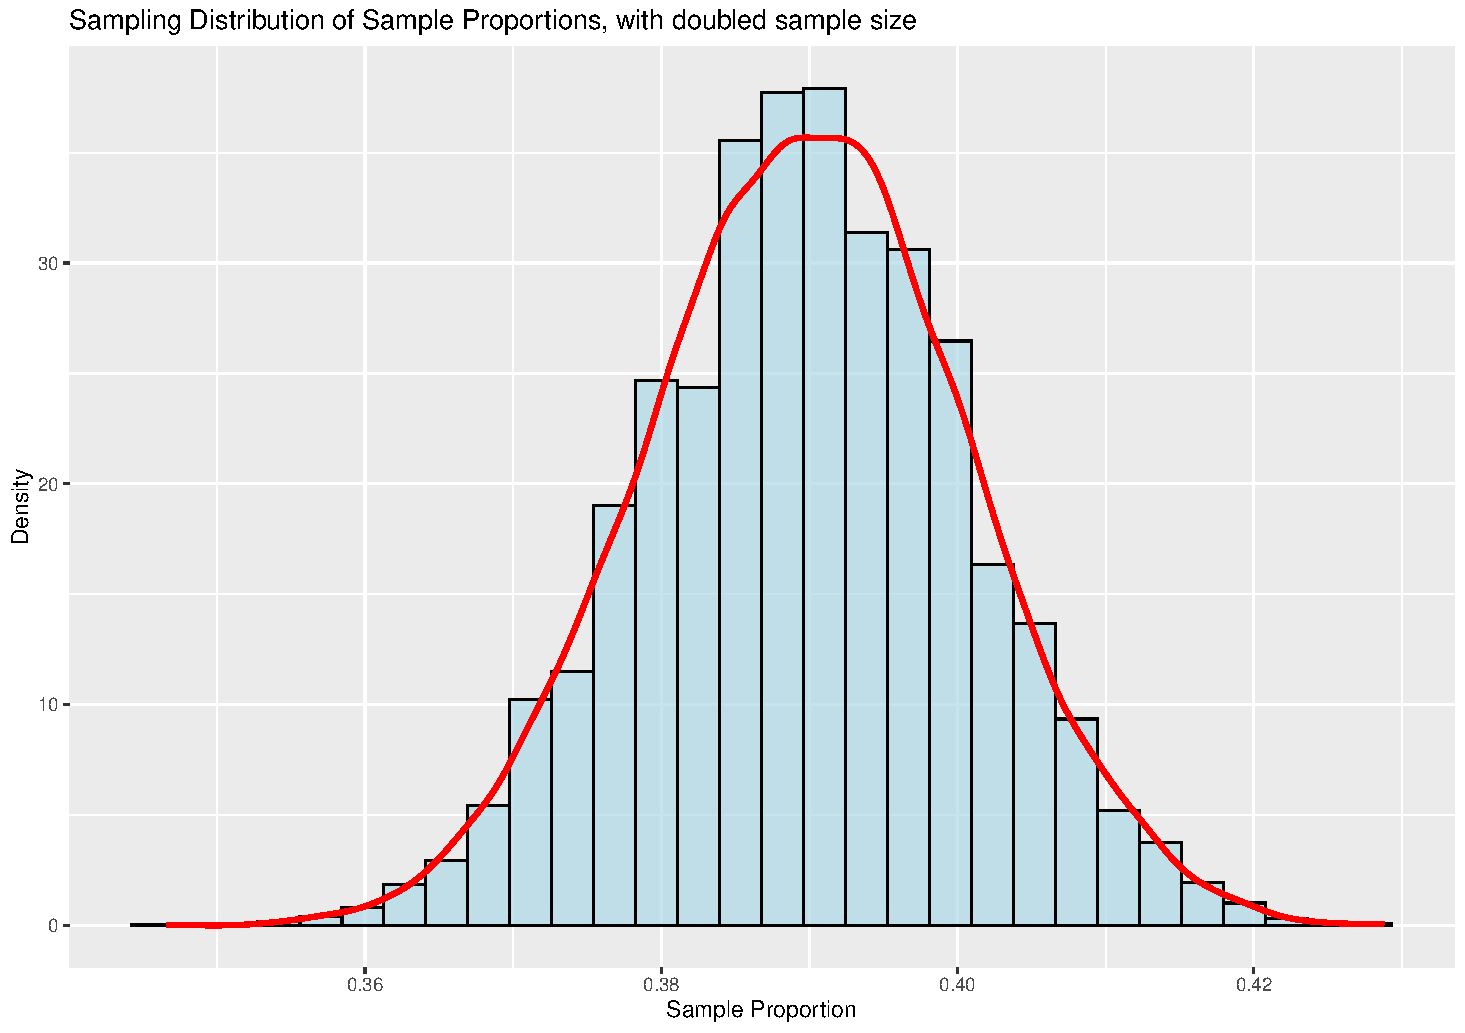
\includegraphics[width=\linewidth]{plot 2.pdf}
\captionof{figure}{Basic Simulation with size 2,008}
\end{Figure}

\section{Resampling}
We generated 1,000 re-samples from the observed Gallup responses (with 39 percent satisfaction and 59 percent unsatisfaction, and one percent not answering). 

\begin{Figure}
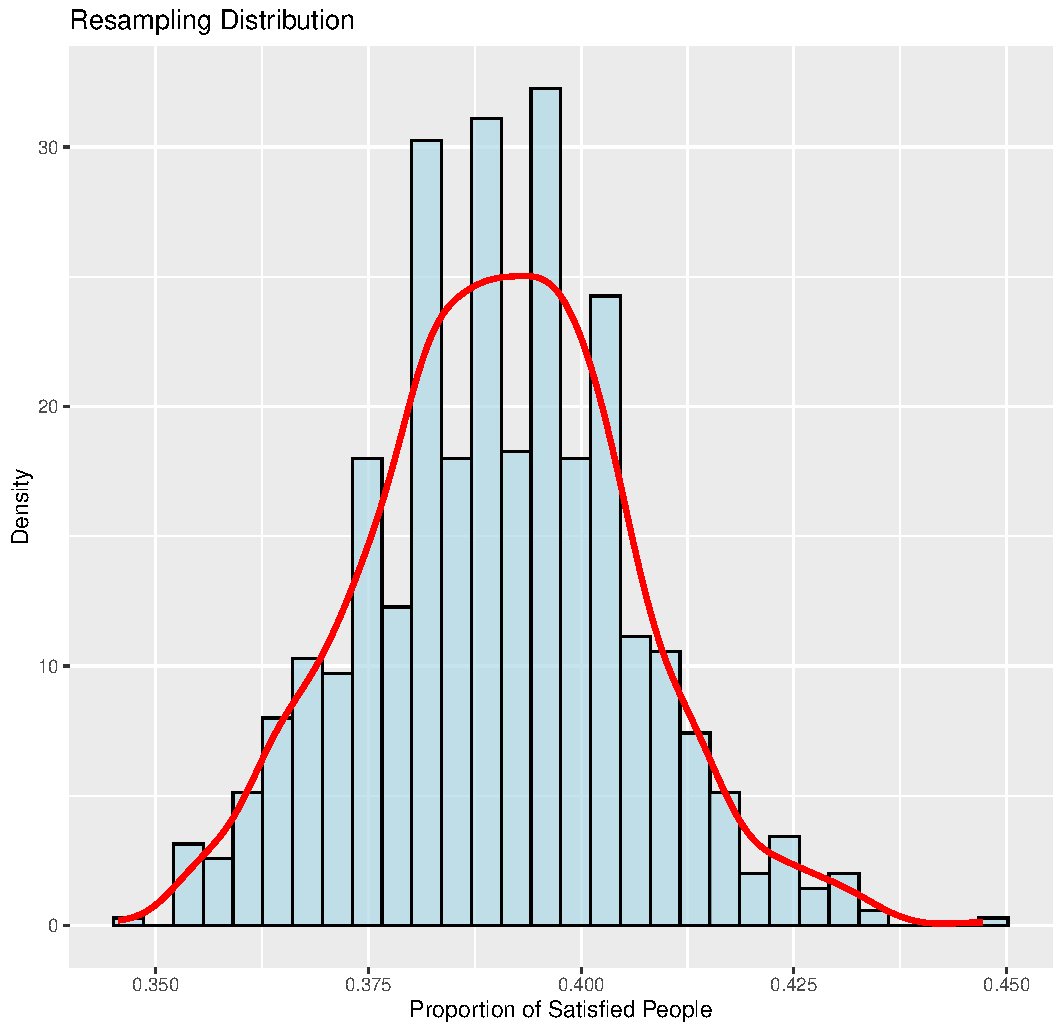
\includegraphics[width=\linewidth]{plot 3.pdf}
\captionof{figure}{Resampling Plot}
\end{Figure}

The resampled margin of error is approximately 2.67 percent, which aligns with the simulaiton results and Gallup's 4 percent margin of error. 

\section{Simulation over n and p}
We simulated 10,000 polls over various values of n and p to estimate margin of error. 

\begin{Figure}
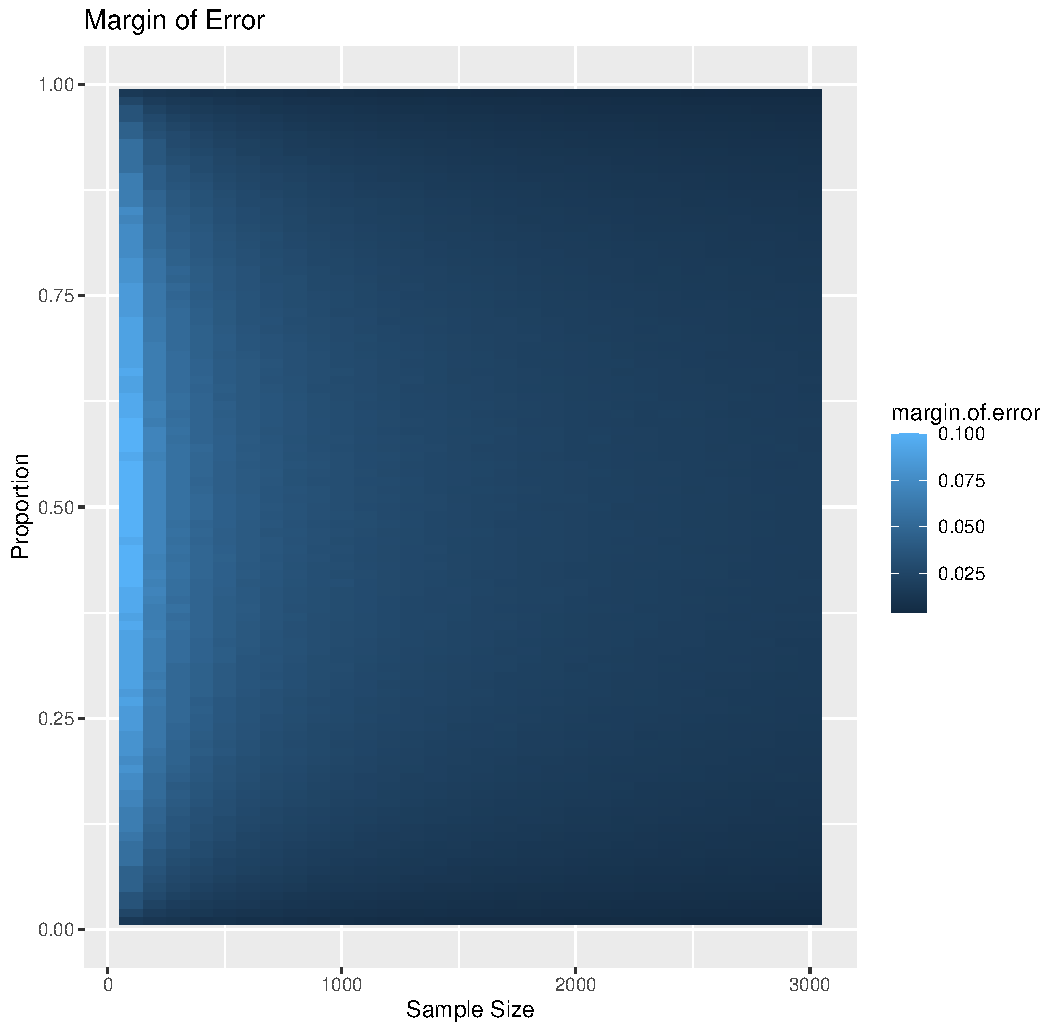
\includegraphics[width=\linewidth]{plot 4.pdf}
\captionof{figure}{Simluation with n and p plot}
\end{Figure}

The margin of error is highest near p equals 0.5, and decreases with bigger samples. This plot could help Gallup understand tradeoffs between cost and accuracy of his experiment. 

\section{Wilson Margin of Error Calculation}
We computed wilson confidence intervals for the same values of n and p.

\begin{Figure}
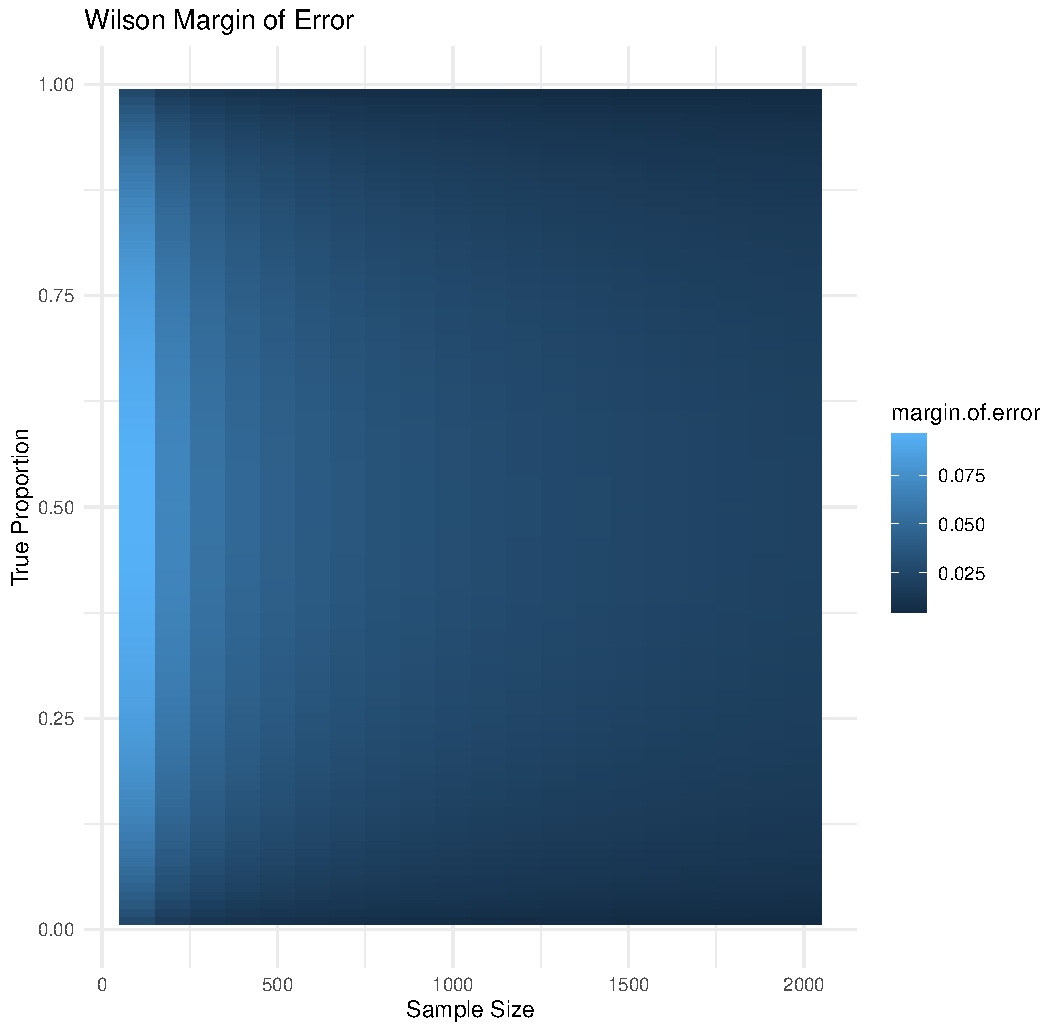
\includegraphics[width=\linewidth]{plot 5.pdf}
\captionof{figure}{Margin of Error}
\end{Figure}

The Wilson margins are similar to simulated ones. This shows that this can be useful when data is really sparse, or when p is extreme. 


\section{Discussion}
Overall, these simulations align with Gallup’s claim about how sample size affects margin of error. Larger samples can lead to smaller margins, and this relationship held true across both basic and resampling methods. The Wilson interval also gave similar results, showing it can be a good alternative, especially when data is limited or when the proportion is very low or high. This lab helped us understand why those who study polls, like Gallup, make choices about sample size and how they try to keep their error low while still being efficient.

%%%%%%%%%%%%%%%%%%%%%%%%%%%%%%%%%%%%%%%%%%%%%%%%%%%%%%%%%%%%%%%%%%%%%%%%%%%%%%%%
% Bibliography
%%%%%%%%%%%%%%%%%%%%%%%%%%%%%%%%%%%%%%%%%%%%%%%%%%%%%%%%%%%%%%%%%%%%%%%%%%%%%%%%
\vspace{2em}

\noindent\textbf{Bibliography:} Note that when you add citations to your bib.bib file \emph{and}
you cite them in your document, the bibliography section will automatically populate here.

\begin{tiny}
\noindent Wickham, H. (2023). \textit{Tidyverse: Easily Install and Load the 'Tidyverse'} [R package version 2.0.0]. Retrieved from \url{https://www.tidyverse.org}

\noindent Gallup, Inc. (2023). \textit{Margin of Error in Polling}. Retrieved from \url{https://news.gallup.com/polling-methodology.aspx}


\end{tiny}
\end{multicols}


\end{document}
